\chapter{Protolib}
\label{protolib}


Protean Protocol Prototyping Library (Protolib) is a low-level 
communication, event dispatching and timing package that 
can be used on top of a network or within the NS-2 network 
simulator environment.  Protolib is not so much a library as it 
is a toolkit.  The goal of the Protolib is to provide a set of simple, 
cross-platform C++ classes that allow development of network 
protocols and applications that can run on different platforms and in 
network simulation environments.  Although Protolib is principally for
research purposes, the code has been constructed to provide
robust, and efficient performance and adaptability to real
applications.

Currently Protolib supports most Unix platforms (including
MacOS X) and WIN32 platforms.  The most recent version also
supports building Protolib-based code for the ns-2 simulation
environment.  The OPNET simulation tool has also been supported
in the past and could be once again with a small amount of
effort.

\index{Ns2}


\section{An overview of Protolib}

\begin{figure}
\centering
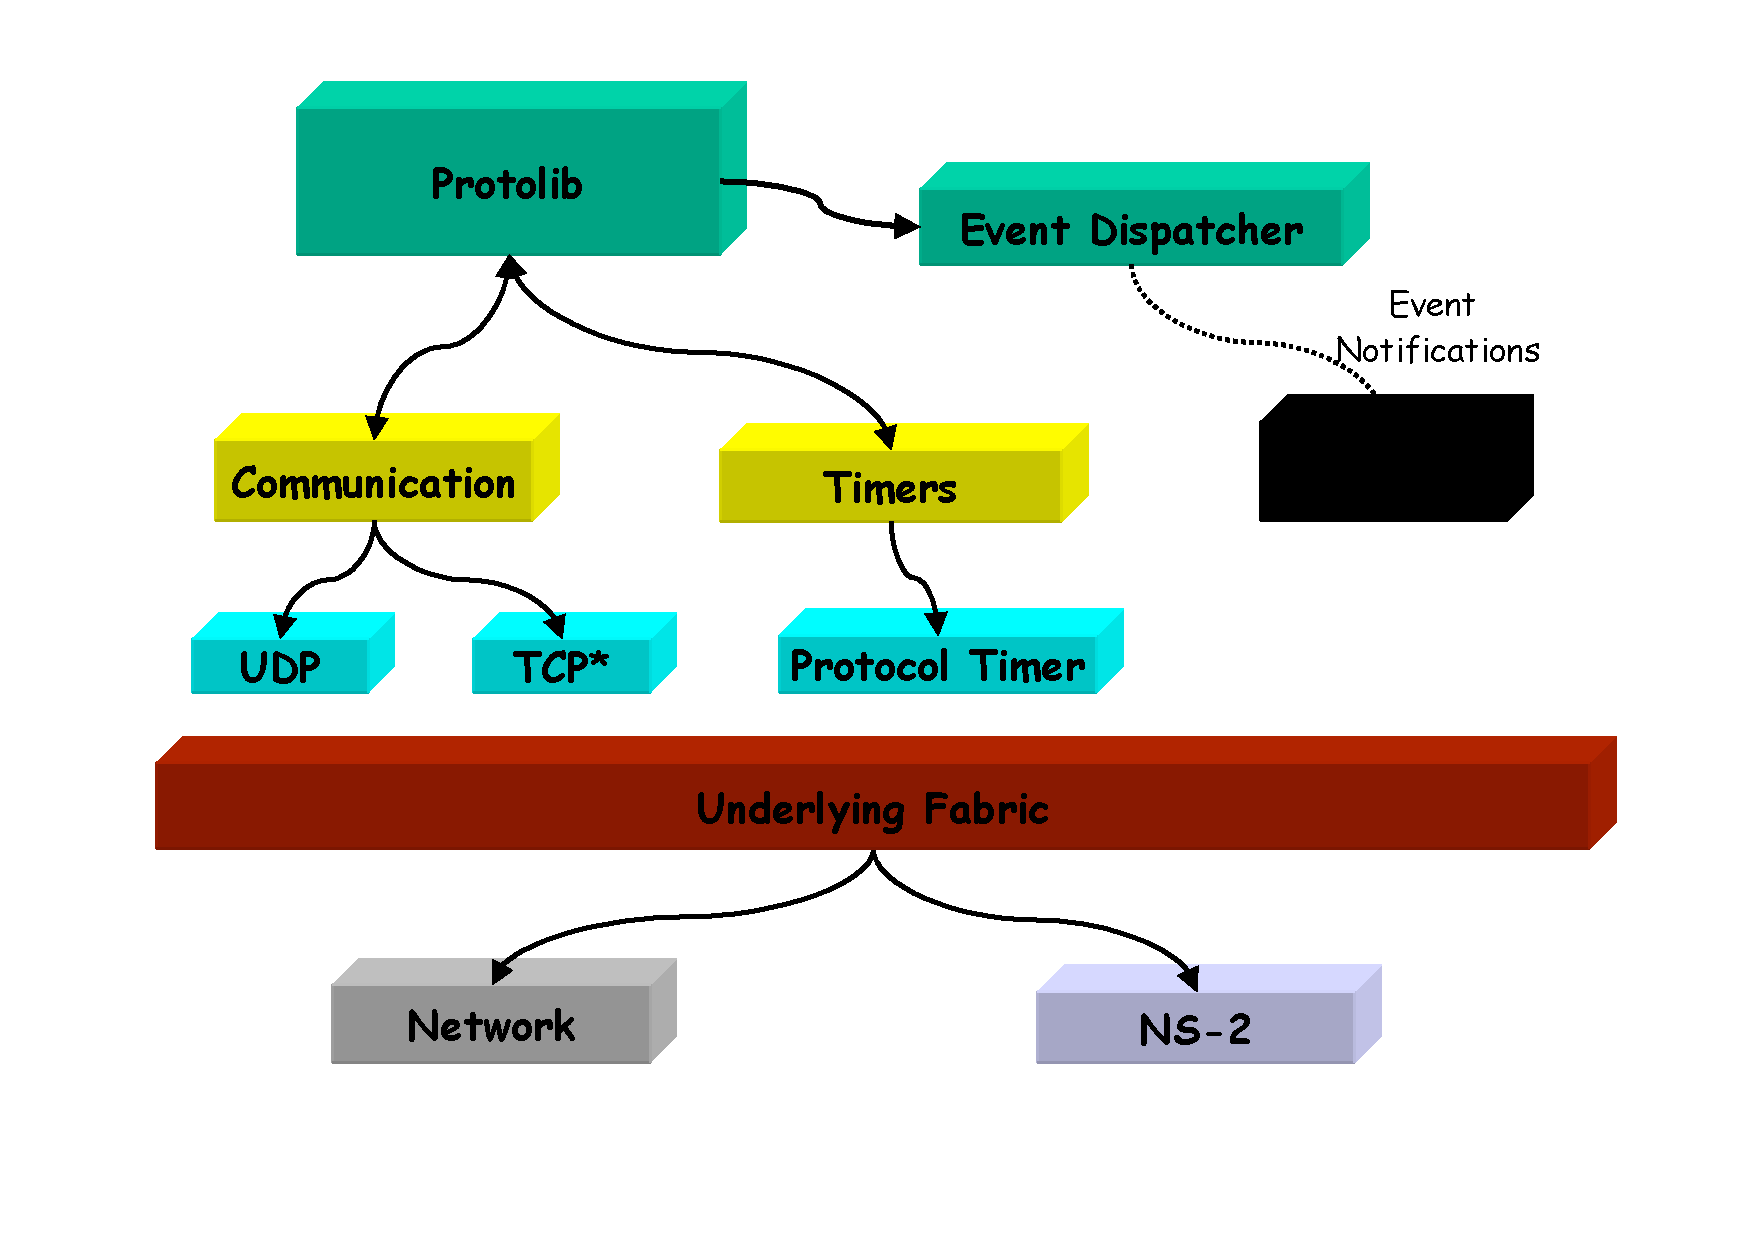
\includegraphics[scale=0.4]{images/protolibOverview}
\caption{An overview of the Protolib toolkit, showing the three distinct 
components, sockets timers and a mechanism for dispatching events.} 
\label{pai:fig:overview}
\end{figure}


A typical usage scenario of Protolib is given in the Fig \ref{pai:fig:demo} . Here, a timer is set up to trigger every 100 milliseconds. Upon a trigger event, a C++ callback is invoked that allows the application developer to integrate an event action. In this example, the application sends a UDP message using Protolib.  This communication mechanism can be achieved using a standard UDP call across a network or between two NS-2 nodes.  When the packet is received by the receiver, another event is generates indicating that data has been received.  This, in turn, calls a routine that allows the application to collect the data from the UDP port and process it in some way. The application interface between the Protolib and the P2P middleware abstracts the reliance on specific networking/timing mechanisms in Protolib to create a generalized pluggable transport mechanism. Within PAI, middleware or indeed applications program to one interface and then choose the environment they want to run within e.g.  Network or NS-2. This is very similar to GATLite but at a far lower level.  PAI also support multiple sockets, timers and corresponding listeners for timeouts or UDP receive data events and establishes a cooperating event dispatching mechanism using multithreading.

\begin{figure}
\centering
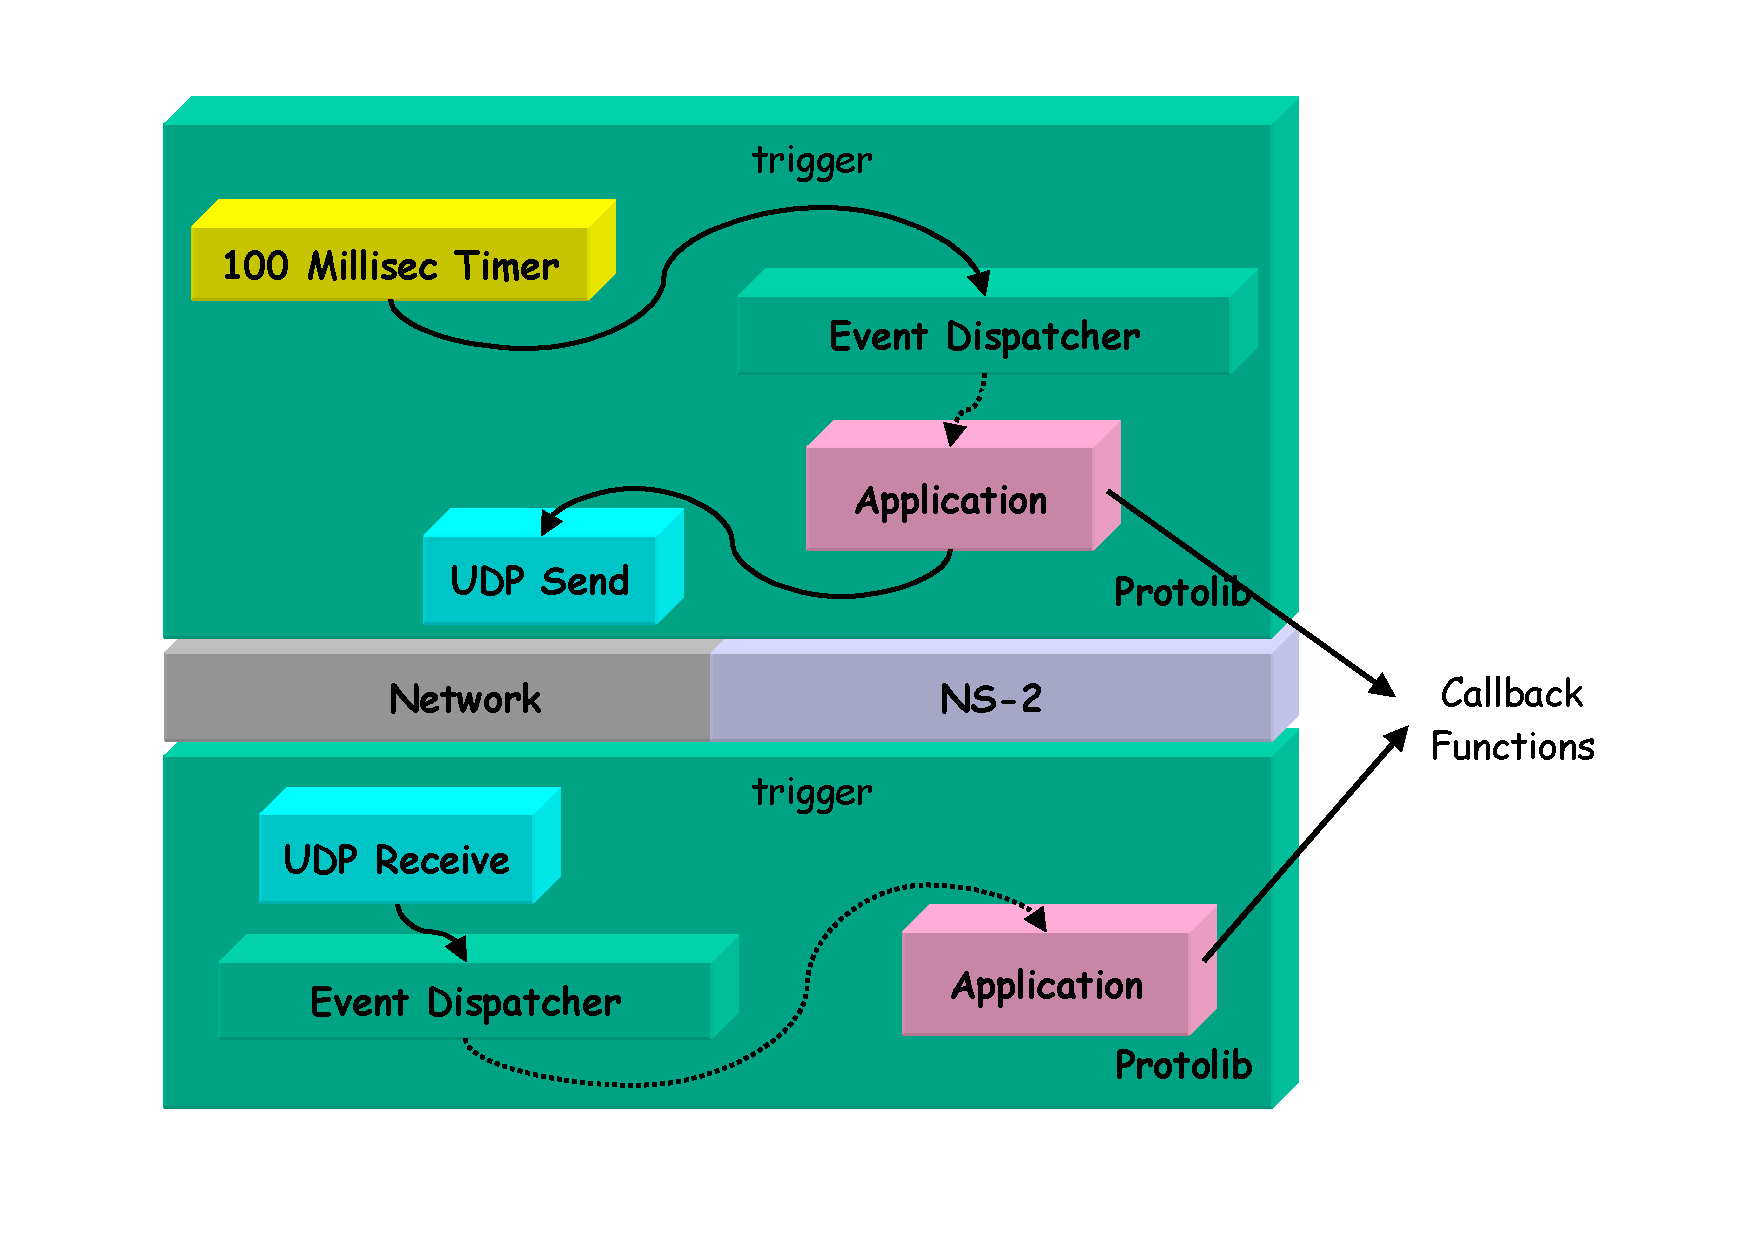
\includegraphics[scale=0.4]{images/protolibDemo}
\caption{An overview of the functionality provided by the ProtoApp
application, which triggers a data send once-per-second.} 
\label{pai:fig:demo}
\end{figure}

\section{Protolib Structure}

The following classes are contained within the Protolib toolkit (taken from the descriptions provide in the release\footnote{Given by Brian Adamson, email: adamson@itd.nrl.navy.mil})

\begin{itemize}
\item \textbf{ProtoAddress:}    Network address container class with support
                 for IPv4, IPv6, and "SIM" address types.  Also
                 includes functions for name/address
                 resolution.

\item \textbf{ProtoSocket:}     Network socket container class that provides
                 consistent interface for use of operating
                 system (or simulation environment) transport
                 sockets. Provides support for asynchronous
                 notification to ProtoSocket::Listeners.  The
                 ProtoSocket class may be used stand-alone, or
                 with other classes described below.  A
                 ProtoSocket may be instantiated as either a
                 UDP or TCP socket.

\item \textbf{ProtoTimer:}      This is a generic timer class which will
                 notify a ProtoTimer::Listener upon timeout.
\item \textbf{ProtoTimerMgr:}   This class manages ProtoTimer instances when
                 they are "activated".  The ProtoDispatcher
                 (below) derives from this to manage
                 ProtoTimers for an application.  (The
                 ProtoSimAgent base class contains a
                 ProtoTimerMgr to similarly manage timers for a
                 simulation instance).

\item \textbf{ProtoTree: }      Flexible implementation of a Patricia tree
                 data structure.  Includes a ProtoTree::Item
                 which may be derived from or used as a
                 container for  whatever data structures and
                 application may require.

\item \textbf{ProtoRouteTable:} Class based on the ProtoTree Patricia tree to
                 store routing table information. Uses the
                 ProtoAddress class to store network routing
                 addresses.  It's a pretty dumbed-down routing
                 table at the moment, but may be enhanced in
                 the future.  Example use of the ProtoTree.

\item \textbf{ProtoRouteMgr:}   Base class for providing  a conistent
                 interface to manage operating system (or
                 other) routing engines.
\item \textbf{ProtoDispatcher:} This class provides a core around which Unix
                 and Win32 applications using Protolib can be
                 implemented.  It's "Run()" method provides a
                 "main loop" which uses the "select()" system
                 call on Unix and the similar
                 "MsgWaitForMultipleObjectsEx()" system call on
                 Win32.  It is planned to eventually provide
                 some built-in support for threading in the
                 future (e.g. the ProtoDispatcher::Run() method
                 might execute in a thread, dispatching events
                 to a parent thread).
\item \textbf{ProtoApp: }       Provides a base class for implementing
                 Protolib-based command-line applications. Note
                 that "ProtoApp" and "ProtoSimAgent" are
                 designed such that subclasses can be derived
                 from either to reuse the same code in either a
                 real-world applications or as an "agent"
                 (entity) within a network simulation
                 environment (e.g. ns-2, OPNET).  A "background"
                 command is included for Win32 to launch the
                 app without a terminal window.

\item \textbf{ProtoSimAgent:}   Base class for simulation agent derivations. 
                 Currently an ns-2 agent base class is derived
                 from this, but it is possible that other
                 simulation environments  (e.g. OPNET, Qualnet)
                 might be supported in a similar fashion.

\item \textbf{NsProtoSimAgent:} Simulation agent base class for creating ns-2
                 instantiations of Protolib-based network
                 protocols and applications.
\item \textbf{ProtoExample:}    Example class which derives either from
                 ProtoApp or NsProtoSimAgent, depending upon
                 compile-time macro definitions.  It provides
                 equivalent functionality in either the
                 simulation environment or as a real-world
                 command-line application.  It demonstrates the
                 use/operation of ProtoSocket based UDP
                 transmission/reception, a ProtoTimer, and an
                 example ProtoSocket-based TCP client-server
                 exchange.   (NOTE: TCP operation is not yet
                 supported in the simulation environment.  This
                 will completed in coming months.  I plan to
                 extend ns-2 TCP agents to support actual
                 transfer of user data to support this.)
\item \textbf{Other:} The Protolib code also includes some simple, general purpose debugging routines which can output to "stderr" or optionally log to a specified file. 
See "protoDebug.h" for details. 

\end{itemize}

\section{Conclusion}


In this chapter, a brief overview of the Protolib toolkit was given.  We gave an overview of its structure and the types of operations it is designed to support (e.g. UDP/TCP communication, timers and event dispatching) and illustrated this through the use of a simple but typical usage scenario. We then gave an overview of the key classes that make up the toolkit. 

Protolib is an evolving toolkit.  As PAI has been integrated on top of Protolib, it has been updated in order to support the functionality required by \agentj~and its applications. PAI, described in the next chapter, focuses on providing the interfaces necessary for Java applications and middleware to use Protolib in a number of different contexts.

